\chapter{Cloud Computing ->Putz}
\putz
%Quellen: Reisi Folien, %Quellen: Reis Folien, https://de.wikipedia.org/wiki/Cloud_Computing#Servicemodelle
\section{Cloud Computing Grundlagen}
\subsection{Definition}
Es gibt einige verschiedene Definitionen des Begriffs \textbf{Cloud Computing}, einer sehr präzise Beschreibung wäre:

\begin{center}
   \textit{Ein Modell zur Bereitstellung von einer Reihe von Services für Unternehmen oder anderweitige Konsumenten über das Internet, wie zum Beispiel das
	Speichern von bestimmten Daten oder das Hosten einer Webseite auf einem Webserver. Die Services sind nicht nur auf Software Angebote beschränkt, es kann zum Beispiel auch Rechenleistung
	angeboten werden. Der Service läuft aus der Sicht des Konsumenten extern beim Anbieter der Services, dem sogenannten Provider.}
\end{center}

Jede Cloud hat bestimmte Eigenschaften welche den Begriff definieren, diese teilen sich in drei Hauptbereiche aus:
\begin{itemize}
	\item die zentralen, essenziellen Charakteristiken einer Cloud
	\item Servicemodelle
	\item Deployment Models oder Bereitstellungsmodelle
\end{itemize}

%Quellen: Reis Folien
%https://de.wikipedia.org/wiki/Cloud_Computing
\subsection{Charakteristiken einer Cloud}
Jede Cloud hat bestimmte spezielle Charakteristiken, das NIST \textbf{(National Institute of Standard and Technology)} listet
momentan fünf essenzielle Eigenschaften die da wären:
\begin{itemize}
	\item \textbf{On-demand self-service: } Bedeutet, dass Ressourcen wie etwa Speicher und Rechenleistung der Cloud, vom Nutzer selbstständig oder automatisiert 
ohne persöhnliche Interaktion mit dem Service Provider in Anpsruch genommen werden kann
	\item \textbf{Broad network access: } Services aus der Cloud sind über das Internet und durch Standardmechanismen, mithilfe von verschiedenen Plattformen wie einem Smartphone, einem Laptop, einem Stand-PC oder Tablet, erreichbar
	\item \textbf{Resource pooling: } Die in generell in einer Cloud zu Verfügung stehenden Ressourcen wie zum Beispiel Speicher und Rechenleistung sind für alle Kunden gebündelt von einem Pool aus verfügbar und werden geteilt, dabei ist der physische Standort der Server für den Klienten in der Regel unbekannt.
	\item \textbf{Rapid elasticity: } Die durch den Kunden in Anspruch genommenen Ressourcen können aus dessen Sicht, schnell ins beinahe unendliche skaliert werden, die Lastenänderung
kann ebenfalls automatisiert angepasst werden, sodass keine menschliche Interaktion notwendig ist.
	\item \textbf{Measured Service: } Die Ressourcennutzung der Kunden kann durch den Anbieter gemessen, überwacht und analysiert werden, zum Zwecke von Abrechnungen, einer effektiver
Nutzung der in Anspruch genommenen Ressourcen oder für eine vorausschauende Gesamtplanung.
\end{itemize}

%Quellen: Reis Folien, https://de.wikipedia.org/wiki/Cloud_Computing#Servicemodelle,
%https://azure.microsoft.com/de-de/overview/what-is-cloud-computing/#cloud-computing-models

\subsection{Servicemodelle}
NIST listet drei grundsätzliche Standard-Modelle, in welcher Form Cloud Computing Dienste angeboten werden können, diese werden oft als Schichten untereinander vereinfacht dargestellt:
\begin{itemize}
	\item Infrastructure as a Service (IaaS)
	\item Platform as a Service (PaaS)
	\item Software as a Service (Saas)
\end{itemize}

%Quellen: Reis Folien, https://de.wikipedia.org/wiki/Cloud_Computing#Servicemodelle,
%https://azure.microsoft.com/de-de/overview/what-is-cloud-computing/#cloud-computing-models,
%https://de.wikipedia.org/wiki/Everything_as_a_Service#Infrastructure_as_a_Service_(IaaS),

\subsubsection{Infrastructure as  a Service (IaaS)}
Bei IaaS nimmt der Kunde IT-Infrastruktur wie Server, Speicher und Virtuelle Computer von einem Cloudanbieter in Anspruch. In diesem Fall gestaltet der Kunde seine eigene Infrastruktur selbst innerhalb einer Cloud und kümmert sich um die Installation von Software und den laufenden Betrieb derer selbst. Der Anbieter ist lediglich für die genutzten physischen Hardware Elemente verantwortlich und wartet diese, alles andere fällt in den Zuständigkeitsbereich des Kunden. Kurz zusammengefasst ist IaaS Bereitstellung von Infrastruktur über das Internet, welche vom Nutzer bedingt kontrolliert wird. \newline
Infrastructure as a Service kann auch als Everything as a Service bezeichnet werden, da in diesem Geschäftsmodell alles vom Kunden selbst verwaltet wird. Einige Charakteristiken von IaaS:
\begin{itemize}
	\item Nur einmalig genutzte Anwendungen werden einmal bezahlt und wieder freigegeben
	\item Im Falle eines explosionsartigen Wachstums und ein erreichen der Belastungsspitzen kann abgefangen werden, da die Services in jede Richtung skalierbar sind. So können innerhalb von Minuten zum Beispiel viel Speicher erweitert werden oder auch im Gegenteil nicht genutzte Kapazitäten frei gegeben werden, welche dann nicht mehr bezahlt werden müssen.
\end{itemize}

Ein Beispiel dafür wäre das Mieten eines VPS-Servers (Virtual Private Server) um eine Webapp wie EMS darauf aufzusetzen.
Als Kunde mietet man eine gewisse Größe an Hauptspeicher (RAM) und Nebenspeicher (SSD), eine Anzahl an CPU-Kernen, wie groß die Bandbreite sein soll und noch viele andere Optionen, welche bei jedem Cloudanbieter variieren. Auf diesem VPS-Server kann man nun sein Front- und Backend aufsetzen und hat über alles selbst die Kontrolle. Klassische Anbieter welche IaaS anbieten wären Amazon mit Amazon Web Services (AWS) mit dem möglicherweise populärsten Service EC2.

%Quellen: Reis Folien, https://de.wikipedia.org/wiki/Cloud_Computing#Servicemodelle,
%https://azure.microsoft.com/de-de/overview/what-is-cloud-computing/#cloud-computing-models,
%https://de.wikipedia.org/wiki/Platform_as_a_Service

\subsubsection{Platform as a Service (PaaS)}
PaaS stellt dem Kunden eine Programmier- und Laufzeitumgebung zur Verfügung. Hier stellt der Cloudanbieter eine Softwareumgebung fertig aufgesetzt für den Nutzer zur Verfügung, damit dieser eigene Softwareanwendungen darauf entwickeln kann. Die Daten- und Rechenkapazitäten der Umgebungen sind dabei flexibel und können somit dynamisch angepasst werden.\newline
\newline
Diese Form des Cloudservices würde sich vor allem an Unternehmen richten, welche eine große Anzahl an Mitarbeiter beschäftigt und an vielen Applikationen gleichzeitig arbeitet und diese schnell entwickeln muss, jedoch nicht genügend Kapital hat, um jeden Arbeitsplatz mit einer Rechenmaschine mit entsprechend benötigter Leistung auszurüsten. Stattdessen könnte solch eine Firma auf PaaS zurückgreifen und für einen geringen Betrag, monatlich diese Umgebungen in einer Cloud mieten und spart sich so viel Kapital und bleibt bei den benötigten Rechenleistungen flexibel, da die Umgebungen eben flexibel auf die benötigten Performanceansprüche skaliert werden kann. Dies wäre bei eingekaufter Hardware in einem Büro nicht so leicht, was dieses Servicemodell den Kunden auch schnell und einfach auf neue Technologien und Anforderungen reagieren lässt.

%Quellen: Reis Folien, https://de.wikipedia.org/wiki/Cloud_Computing#Servicemodelle,
%https://azure.microsoft.com/de-de/overview/what-is-cloud-computing/#cloud-computing-models,
%https://de.wikipedia.org/wiki/Software_as_a_Service

\subsubsection{Software as a Service (SaaS)}
Manchmal auf als Software on Demand beschrieben, was "`Software nach Bedarf"' übersetzt bedeutet. Hier bietet der Cloudanbieter spezielle Software zur Nutzung an. Der Kunde kann dann diese Software- und Anwendungsprogramme nach belieben benutzen. Die Applikationen werden über das Internet dem Nutzer zur Verfügung gestellt, und dieser kann mittels einer API darauf zugreifen, was meistens über einen Browser oder eine App geschieht. Die Infrastruktur hinter den Anwendungen verwaltet der Anbieter selbst und auch die angebotene Software könnte nur bis zu einem gewissen Teil vom Kunden konfiguriert werden. Also sämtliche Instandhaltungsarbeiten obliegen dem Cloudanbieter. Der Nutzer benutzt lediglich die angebotene Software und kann sich bei Problemen nur an den Support wenden.\newline
\newline
Ein Beispiel für so ein Service, wären die meisten Google Services wie Gmail, Docs, Drive und Photos. Noch weitere prominente Beispiele für Software as a Service, sind Github, Office 365 und Dropbox.\newline

Zusätzlich zu den oben genannten standardisierten Modellen, existieren noch einige weitere Modelle auf dem Markt. Prinzipiell
kann man heutzutage fast jeden nur denkbaren Service über eine Cloud beziehen, mit der Zeit haben sich dafür spezielle Bezeichnungen gebildet. Diese Fachbegriffe können zusammengefasst werden:
\begin{itemize}
	\item Function as a Service (FaaS)
	\item Everything as a Service (XaaS)
\end{itemize}

%Quellen: Reis Folien, https://de.wikipedia.org/wiki/Cloud_Computing#Servicemodelle,
%https://azure.microsoft.com/de-de/overview/what-is-cloud-computing/#cloud-computing-models,
%https://de.wikipedia.org/wiki/Function_as_a_Service

\subsubsection{Function as a Service (FaaS)}
Prinzipiell ist FaaS von den Angeboten und Leistungen ähnlich wie das vorhin beschriebene Paas-Modell. Es stellt eine Laufzeitumgebung zur Verfügung, worauf Softwareanwendungen erstellt werden könne. Der maßgebende Unterschied zwischen Function und Platform as a Service ist, dass bei PaaS die Skalierung mittels hinzufügen von weiteren Serverprozessen zu den bereits in Anspruch genommenen stattfindet. Dies bewirkt natürlich normalerweise eine Kostenerhöhung auf Seiten des Benutzers, welche direkt Abgebucht oder in Rechnung gestellt wird. Die Skalierung ist dem Benutzer hier dadurch aber auch sehr übersichtlich und man kann die Aus- und Belastung seiner Entwicklerumgebung leicht nachvollziehen.\newline
Ganz anders im Gegensatz dazu geschieht die Skalierung bei FaaS. Bei diesem Service läuft keine extra Serverinstanz im Hintergrund. Bei FaaS muss der Benutzer die \textbf{Function exceution time} bezahlen. Die Zeit zwischen den Ausführungen von Code wird hierbei nicht in Rechnung gestellt, also lediglich, wenn ein Code zum Beispiel übersetzt oder ein Programm ausgeführt und getestet wird. Somit muss der Benutzer auch nicht mehr an die Skalierung denken, da seine Entwicklerumgebung quasi kostenlos zu Verfügung steht und er nur die Ausführung der Software nach deren Zeitaufwand bezahlen muss. Dies sorgt für geringere Kosten auf Seiten des Kunden, bei gleichzeitig höhere Skalierbarkeit, da diese nicht mehr beachtet werden muss. Einen Nachteil gibt es jedoch und zwar kann die Latenz bei diesem Server höher als bei einer Lösung mit PaaS sein. Dies ist jedoch von vielen Faktoren und nicht zuletzt auch von der Komplexität des kodierten Programmes abhängig.

Dieser Service verfolgt den Ansatz des sogenannten \textbf{"`serverless computing"'}. Hierbei übernimmt der Cloud-Anbieter die komplette Ressourcenzuweisung, zum Beispiel benötigter Speicher und benötigte Prozessorkernanzahl, für den Kunden. Bei serverless computing wird keine Ressource im volatilen Speicher gehalten. Dies bedeutet, Berechnungen werden in bestimmten Abständen durch bestimmte Events von Seiten des Kunden aus, ausgelöst und die Ergebnisse werden dann in einen persistenten Speicher geschrieben. Wenn eine Anwendung gerade nicht vom Kunden benutzt wird, wird dies auch nicht in Rechnung gestellt wie es bei herkömmlichen Services der Fall ist. Es gibt keinen fixierten Betrag der monatlich oder Quartals mäßig abgebucht wird, sondern nur produktiv genutzte Zeit in der Anwendung wird berechnet.

Das erste offizielle, kommerzielle Angebot eines solchen Services gab es 2006. Seitdem haben viele große Cloud-Anbieter wie zum Beispiel Amazon mit AWS Lambda, Google und Microsoft mit Azure, solche \textbf{pay as you go} Services zu Verfügung gestellt.


% Quellen: https://www.quora.com/What-are-the-Iaas-Paas-and-SaaS-services-in-Amazon-webservices?share=1
%https://de.wikipedia.org/wiki/Everything_as_a_Service#Weitere_Ans%C3%A4tze_2
%https://web.archive.org/web/20110728093045/http://www.thecloudcomputing.org/2009/1/panels.html#Panel2

\subsubsection{Everything as a Service (XaaS)}
XaaS oder auch EaaS, stellt prinzipiell alles zu Verfügung. Also SaaS, Paas sowie auch Iaas. Einige Anbieter spezialisieren sich auf ein bestimmtes Service Modell, manche bieten jedoch prinzipiell alle Services unter der Bezeichnung XaaS an und spalten diese Services in die spezifischere Modelle, wie zum Beispiel SaaS, auf. Dies sorgt vor allem bei Neukunden manchmal für Verwirrung. AWS (Amazon Webservices) ist so ein Service, er bietet prinzipiell jedes Modell unter XaaS an, jedoch sind hunderte weitere Services einzeln spezifiziert verfügbar. AWS heißt lediglich das Cloud Computing System, ein tatsächlicher Service heißt zum Beispiel AWS EC2, dieser Service ist als IaaS zu spezifizieren. Hierbei kann man einen virtuellen Server mit einem bestimmten Betriebssystem, virtuelle Kernanzahl und Hauptspeicher mieten. Dieser Service kostet stündlich, egal ob er benutzt wird oder nicht. Ein weitere IaaS Service in AWS ist S3, hier kann man Speicher mieten.\newline
AWS bietet stand April 2021 über 200 verschiedenen Services in allen Servicemodellen Iaas, Paas und SaaS.
\newline
Weitere noch spezifischere Servicemodelle wie zum Beispiel High Performance Computing as a Service (HPCaaS), Data Intensive Computing as a Service (DICaaS) oder Humans as a Service (HuaaS). Können unter XaaS übergeordnet zusammengefasst werden. Für HuaaS als Beispiel gibt es den AWS Service Amazon Mechanical Turk, dieser Dienst befindet sich jedoch noch in einer Beta-Phase, hierbei wird menschliche Intelligenz wie ein Webservice genutzt.

%Quellen:
%Reis Folien
%https://de.wikipedia.org/wiki/Cloud_Computing#Organisatorische_Arten_von_Clouds
\subsection{Liefermodelle}
Im Kapitel Servicemodelle (Sektion 1.1.3) wurde die verschiedenen Modelle, welche eine Cloud anbieten kann und wie viele gleiche Hardwareeinheiten, beginnend mit der Aufteilung derer Infrastruktur bis zur Verfügungstellung einzelner Endanwendungen, für den Endkunden benutzbar gemacht wird.\newline
Im Englischen werden sie \textbf{Deployment Models} genannt, die im deutsch genannten Liefermodelle beschreiben nun, wie genau die Services unter Berücksichtigung ihrer Aufteilung in bereits genannte Servicemodelle, einem Benutzer zu Verfügung gestellt werden:
\begin{itemize}
	\item Private cloud
	\item Public cloud
	\item Hybrid cloud
	\item Community cloud
\end{itemize}

\begin{center}
\begin{figure}[h]
    \centering
    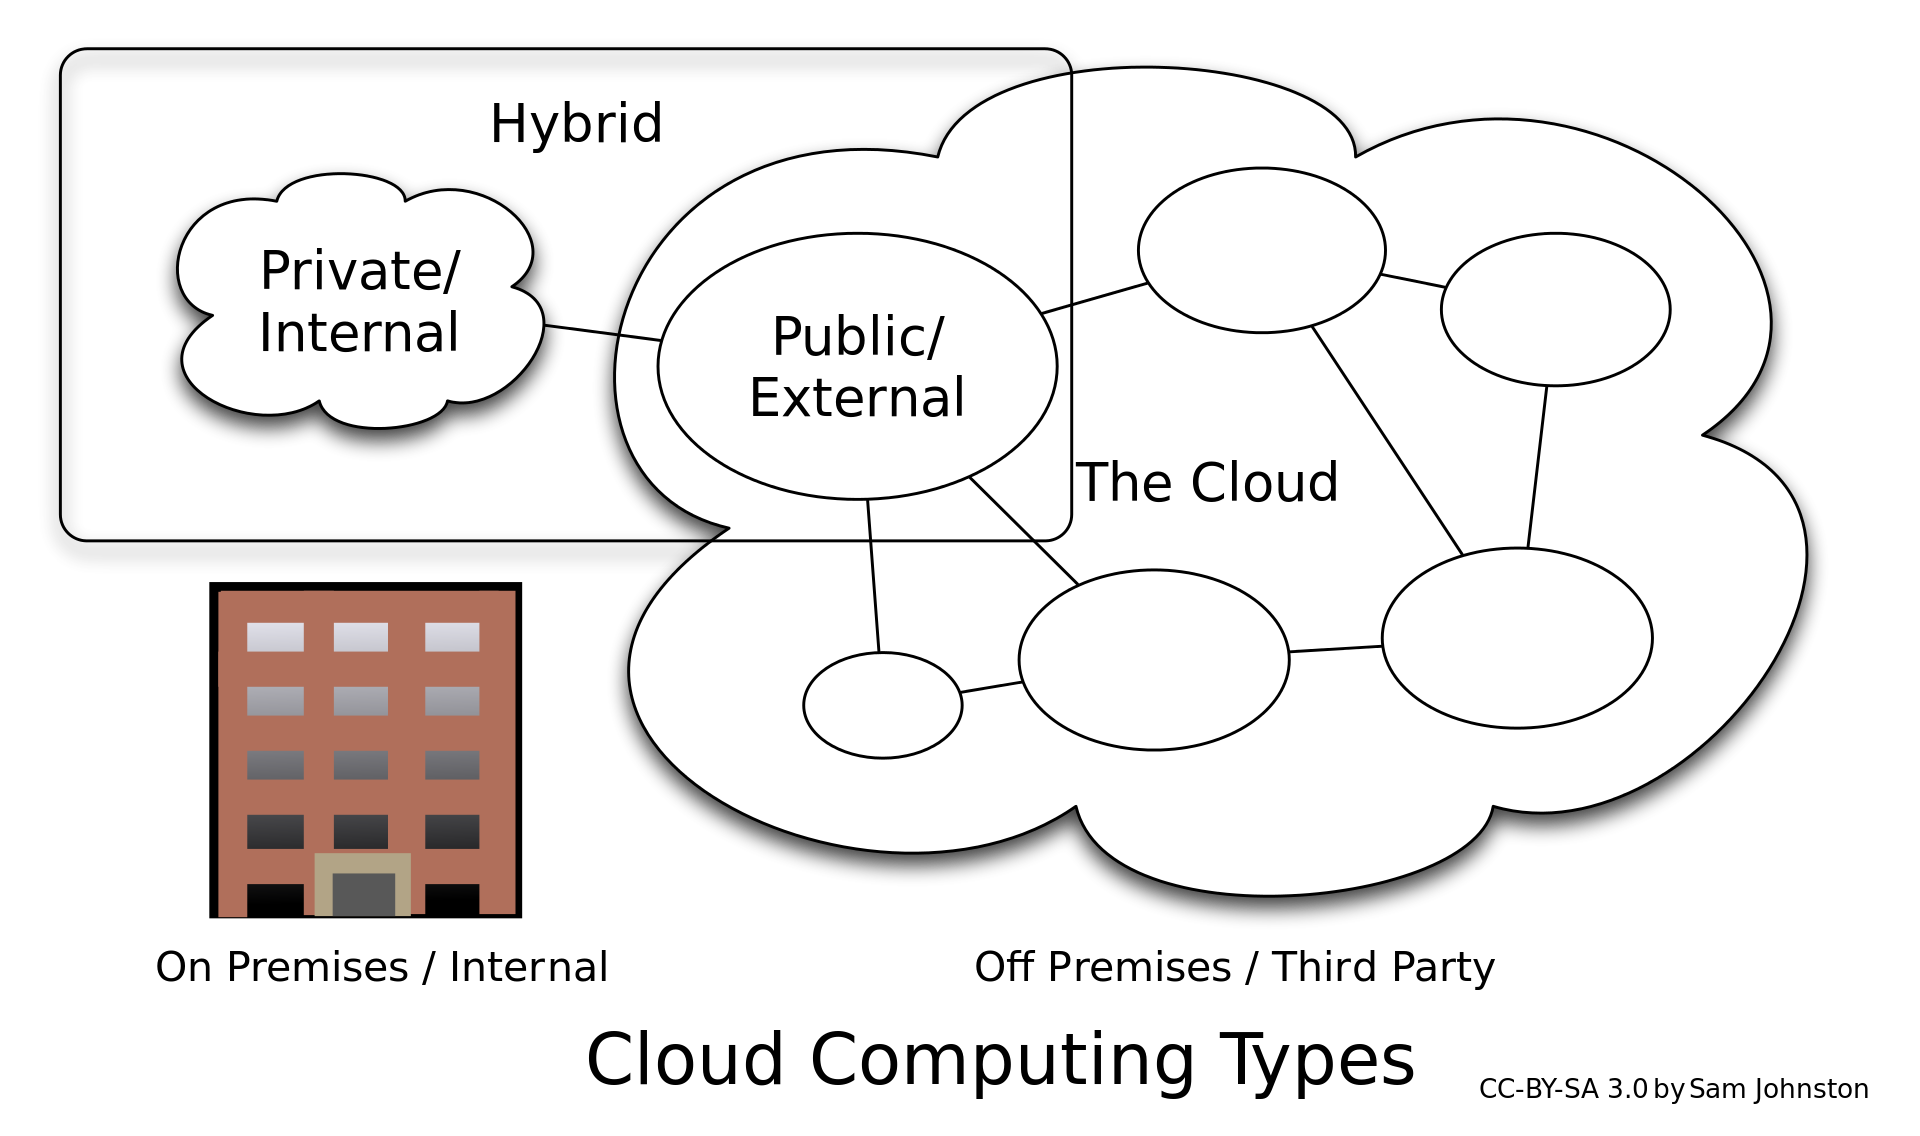
\includegraphics[width=\textwidth]{Cloud_computing_types.png}
    \caption{Liefermodelle von Cloud Computing}
\end{figure}
\end{center}

%Quellen:
%Reis Folien
%https://de.wikipedia.org/wiki/Cloud_Computing#Organisatorische_Arten_von_Clouds
%https://azure.microsoft.com/en-us/overview/what-is-a-private-cloud/
\subsubsection{Private cloud}
Private Clouds werden nur von einem einzelnen Unternehmen, einer Organisation oder einem Kunden betrieben oder stehen nur diesen und einem vertrauenswürdigen Dritten zu Verfügung. Diese Cloud-Umgebung wird entweder intern von zum Beispiel in einem firmeneigenen Rechenzentrum gehostet und verwaltet, oder aber der vertrauenswürdige Dritte übernimmt das Hosting. In letzterem Fall liegt das Rechenzentrum extern bei dem Dritten. Nicht zu verwechseln mit einem normalen IT-Betrieb, wie er in fast jedem kleinen bis mittleren Unternehmen betrieben wird. Die Bezeichnung \textbf{Private cloud} ist erst dann zutreffend, wenn alle fünf Charakteristika einer Cloud erfüllt werden (siehe Kapitel 1.1.2).
Bei einer privaten Cloud gibt es verschiedene Evolutionsstufen, welche die Wichtigkeit beziehungsweise die Verbreitung und den Nutzungsgrad innerhalb der Organisation beschreibt:
\begin{itemize}
	\item Exploratory cloud: Hier wird die Private Cloud hauptsächlich als Testumgebung parallel zum Produktivbetrieb genutzt. Oft wird sie auch, falls man sich Know-how im Gebiet des Cloud Computing anschaffen will, für Studien um Potential und Nachteilen einer internen Cloud herauszufinden, benutzt.
	\item Department cloud: Eine Cloud, die vor allem produktiv und abteilungsintern genutzt wird.
	\item Enterprise cloud: Diese Form der privaten Cloud wird im gesamten Unternehmen benutzt und ist fest im Produktivbetrieb integriert.
\end{itemize}

Microsoft bietet mit Azure einen Service an, nämlich \textbf{Azure Express Route}, welcher vor allem auf Ansprüche einer Private cloud angepasst ist.
Anwendungsfälle für eine private Cloud gibt es vor allem in Unternehmen, welche Daten speichert oder verarbeitet, welche im Rahmen der DSGVO unter den Begriff \textbf{sensible Daten} fällt.

%Quellen:
%Reis Folien
%https://azure.microsoft.com/en-us/overview/what-are-private-public-hybrid-clouds/
\subsubsection{Public cloud}
Eine Public Cloud für die breite Öffentlichkeit und Einzelpersonen einen Zugang zu ihren Services über das Internet. Die Kunden von Anbieter, welche eine Public Cloud betreiben, können somit jeder mit einem Internetzugang sein. Eine öffentliche Cloud kann mit drei weitere Formen genauer aufteilen:
\begin{itemize}
	\item Exclusive Cloud: Der Benutzer/Kunde und der Hoster der Cloud kennen sich persönlich durch zum Beispiel Schriftverkehr (E-Mail). Normalerweise besteht zwischen den Parteien ein individueller bilateraler Vertrag
	\item Open Cloud: In der Regel kennen sich der Benutzer/Kunde und Cloudanbieter nicht. In sogenannten \textbf{"`Service Level Agreements"'}, oder kurz SSL, werden die Leistungen und die Vergütung jeder genauestens beschrieben. Hier laufen Vertragsabschluss und Nutzung voll- oder teilautomatisiert ab, da die Anzahl der Nutzer bei dieser Form der öffentlichen Cloud viel höher als bei allen anderen ist.
	\item Virtual Private Cloud: Ein abgetrennter Bereich in einer öffentlichen Cloud, der für einen bestimmten einzelnen Kunden reserviert wird. Zusätzlich werden durch besondere Sicherheitsmaßnahmen entsprechende Vorkehrungen, für die Integrität des exklusiven Bereichs sorgen, getroffen. Ein Beispiel wäre bei Inanspruchnahme eines IaaS, die physische Trennung der gemieteten Hardware von der restlichen oder bei anderen Services ein spezieller Zugang über einen VPN.
\end{itemize}

Die bekanntesten öffentlichen Clouds sind Amazon Web Services, Google App Engine, Windows Azure und auch Salesforce.

%Quellen:
%Reis Folien
%https://de.wikipedia.org/wiki/Cloud_Computing#Organisatorische_Arten_von_Clouds
%https://en.wikipedia.org/wiki/Cloud_computing#Serverless_computing
\subsubsection{Hybrid cloud}
Das Konzept einer Hybriden Cloud besteht aus einer Mischung aus privater, öffentlicher und Community Cloud. Ein Beispiel für die Anwendung einer solchen Form wäre zum Beispiel, ein Unternehmen hat eine private Enterprise Cloud, und nutzt aber zusätzlich als Backup falls es zum Beispiel die Belastungsspitze des System erreicht wird, eine öffentliche oder Community Cloud.

%Quellen:
%Reis Folien
%https://de.wikipedia.org/wiki/Cloud_Computing#Organisatorische_Arten_von_Clouds
%https://en.wikipedia.org/wiki/Cloud_computing#Serverless_computing
\subsubsection{Community cloud}
Eine Community Cloud ist ein Zusammenschluss von einigen unter sich bekannter Nutzer. Diese "`verschmolzene"' neue Cloud aus zum Beispiel einiger privaten Clouds welche einen sehr ähnlichen oder gleichen Zweck hatten, kann intern in deren Gebäuden gehostet werden, oder extern von einem Dritten betrieben werden. Die Kosten dafür wird unter den ursprünglichen Teilnehmern aufgeteilt.
Ein Anbieter hierfür wäre zum Beispiel \textbf{Googel Gov Cloud}.

\section{Cloud Computing Wirtschaftlichkeit}
Cloud Computing bietet generell viele Möglichkeiten und bringt viele Vorteile mit sich, welche mit einer klassischen Unternehmes-IT von mittlere bis großen Betrieben nicht möglich sind. Vor allem auch die Analyse von Big Data und die exponentiell ansteigende Menge an zu verarbeitenden Daten, wären ohne Cloud Lösung nicht in diesem Umfang wie er im momentanen stattfindet, möglich.
Eine Cloud Lösung bietet aber nicht immer einen Mehrwert. Viele kleine und mittleren Betriebe müssen genau abwiegen, ob in ihrem speziellen Fall eine Lösung mittels Cloud Computing, wirtschaftlich und ressourcentechnisch sinnvoll wäre.
Um die Vorteile, Nachteile und Möglichkeiten bei der Nutzung von Cloud Computing abzuwiegen, kann man eine sogenannte SWOT-Analyse
durchführen:
\begin{itemize}
	\item \textbf{S}trength
	\item \textbf{W}eakness
	\item \textbf{O}pportunity
	\item \textbf{T}ransition
\end{itemize}

\paragraph{Strength (Stärken):} In diesem Teil der Analyse werden die Stärken/Vorteile einer Cloud Lösung im Gegensatz zu einer internen IT-Lösung betrachtet. Hier sticht vor allem heraus, das die Stärken einer Cloud in der Verfügbarkeit, Stabilität, Performance und letzten Endes vor allem in der Skalierbarkeit liegen. Zum Beispiel, falls bei einer intern gewählten Hardwarelöung, die maximale Nutzlast der Server ständig erreicht wird, kann sich das negativ auf die Performance und somit die Kundenzufriedenheit, und der Lebensdauer der Hardwareteile auswirken. Bei einer Cloud-Lösung kann hier einfach per Knopfdruck im Notfall manuell, oder auch vollautomatisiert auf zum Beispiel prozentualer Auslastung, einfach nach oben skaliert werden. Ist der Ansturm vorbei, können nicht benötigte Ressourcen wieder freigegeben werden.
Bei einer internen Lösung wie vorhin beschrieben, wäre dies nicht so einfach möglich, da zuerst teure Hardware eingekauft, geliefert und auch installiert werden müsste.\\

\paragraph{Weakness (Schwächen):} Außer die Nachteile in bestimmten Use-Cases, hat Cloud Computing außerdem ein paar andere Schwächen im Gegensatz zu einer internen Lösung. Einerseits kauft man sich die IT-Kompetenz ein, dies kann gleichzeitig zwar auch ein Vorteil sein, da man sich in erster Linie Geld und Zeit spart im Falle einer Anschaffung, jedoch entsteht eine gewisse Abhängigkeit zum Anbieter des in Anspruch genommenen Services. Bei Cloud Computing werden noch weitere Freiheiten im Gegensatz für Kostenreduzierung aufgegeben. Der Kunde muss sich auf die Zuverlässigkeit der Kommunikation und der durchgehenden Verfügbarkeit seines Services verlassen. Weiters differenziert man sich weniger von der Konkurrenz, welche den gleichen Anbieter nutzen, da dieselbe Software und/oder Infrastruktur verwendet wird, da gleicher Cloud Anbieter.\\

\paragraph{Opportunity (Gelegenheiten):} Außer den bei Stärken genannten positiven Eigenschaften, bringen Cloud Lösungen einige neue und innovative Gelegenheiten mit sich. Einerseits verkürzt sich die time-to-market, da in einer Cloud Umgebung schneller entwickelt werden kann und die Services untereinander sehr gut auf einander abgestimmt sind, um möglichst kurze Entwicklungszeiten einzelner Releases zu unterstützen. Ein weiterer wirtschatlicher Aspekt ist das Economies of scale. Die Lizenzkosten für Betriebssystem, Hardware und andere Software, sind bei Einzelanschaffung recht hoch. Die Kosten für Wartung und Instandhaltung müssen von jedem selbst getragen werden, sowie Updates im Bezug auf Sicherheit. Diese Kosten sind redundant, legt man jedoch viele Rechenzentren zu einem einzelnen zusammen, schafft eine Cloud und lässt mehr Benutzer auf das gleiche System zugreifen, senkt dies Anschaffungs- und Erhaltungskosten drastisch nach dem Prinzip "´buy more pay less"'. Dies ist in Abb. XX gut veranschaulicht, hier sieht man die Benutzerzahlen einer Cloud im Verhältnis zu den Kosten pro Person für die Anschaffung.\\

\paragraph{Transition (Risiken):} Cloud Computing bringt vor allem im Bezug auf den Datenschutz ein großes Risiko auf. Viele Daten werden nicht in der EU gelagert. Sieben von Zehn kommerziellen Rechenzentren haben ihren Standort in den USA und unterliegen somit auch den Datenschutzrichtlinien in diesem Land. Für sämtliche Daten welche in der EU gesammelt und/oder verarbeitet werden, gibt es bestimmte Richtlinien und Gesetzte, vor allem für die Übertragung ins Ausland (Kapitel 2). Dies bewirkt einen großen Aufwand und benötigt bei manchen Unternehmen, ausgehend vom Ort der Sammlung der zu verarbeitenden Daten, Individuallösungen. Ein weiteres Risiko ist die Abhängigkeit die zum Anbieter entsteht, ständig Systeme von einem zu einem anderen zu migrieren ist aufwändig und auf lange Sicht nicht wirtschaftlich, dies sollte man vermeiden. Ein weiterer Punkt welcher unbedingt auch festegelegt werden muss ist, welche Seite für Backups verantwortlich ist, deren Zeitspannen, Häufigkeit, Integrität und Aufbewahrungsdauer. Auch hier spielt der Datenschutz eine wichtige zu beachtende Rolle.

\begin{center}
\begin{figure}[h]
    \centering
    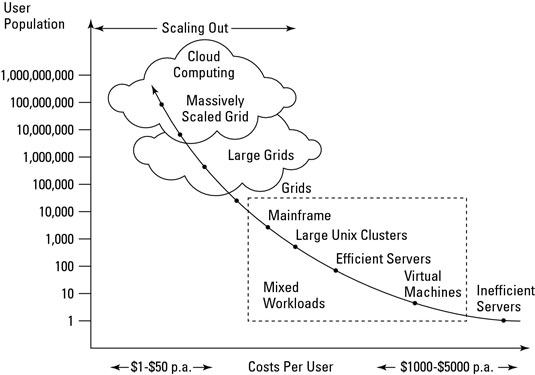
\includegraphics[width=\textwidth]{eos.png}
    \caption{Economies of Scale}
\end{figure}
\end{center}
\break

%https://ourcodeworld.com/articles/read/977/how-to-deploy-a-node-js-application-on-aws-ec2-server
\section{Cloud Anbieter AWS}
Bei EMS wurde sich nach einigen Abwägungen für das Cloud Computing System von Amazon, AWS, entschieden. Neben der einhergehenden Popularität des Anbieters spielten auch vor allem die Preise, einfache automatisierte Skalierbarkeit und bereits vorhandenes Know-How im deployen von Full-Stack Anwendungen auf den Service EC2, eine Rolle bei der Wahl.

\subsection{Erstellen einer EC2 Instanz}
Nachdem auf der Webseite von Aamzon Web Services ein Account erstellt worden ist, gelangt man auf die Homepage für verifizierte Benutzer. Auf der linken oberen Ecke unter Services (Abb. XX), findet man sämtliche Cloud Lösungen welche AWS bietet, stand bei Verfassung dieser Schrift, über 200. Im rechten roten Kreis, sieht man zugleich den Servce "´EC2"', welcher hierfür relevant ist, falls dieser nicht angezeigt wird, kann man oben in der Suchleiste den Namen des gesuchten AWS Services eingeben.

\begin{center}
\begin{figure}[h]
    \centering
    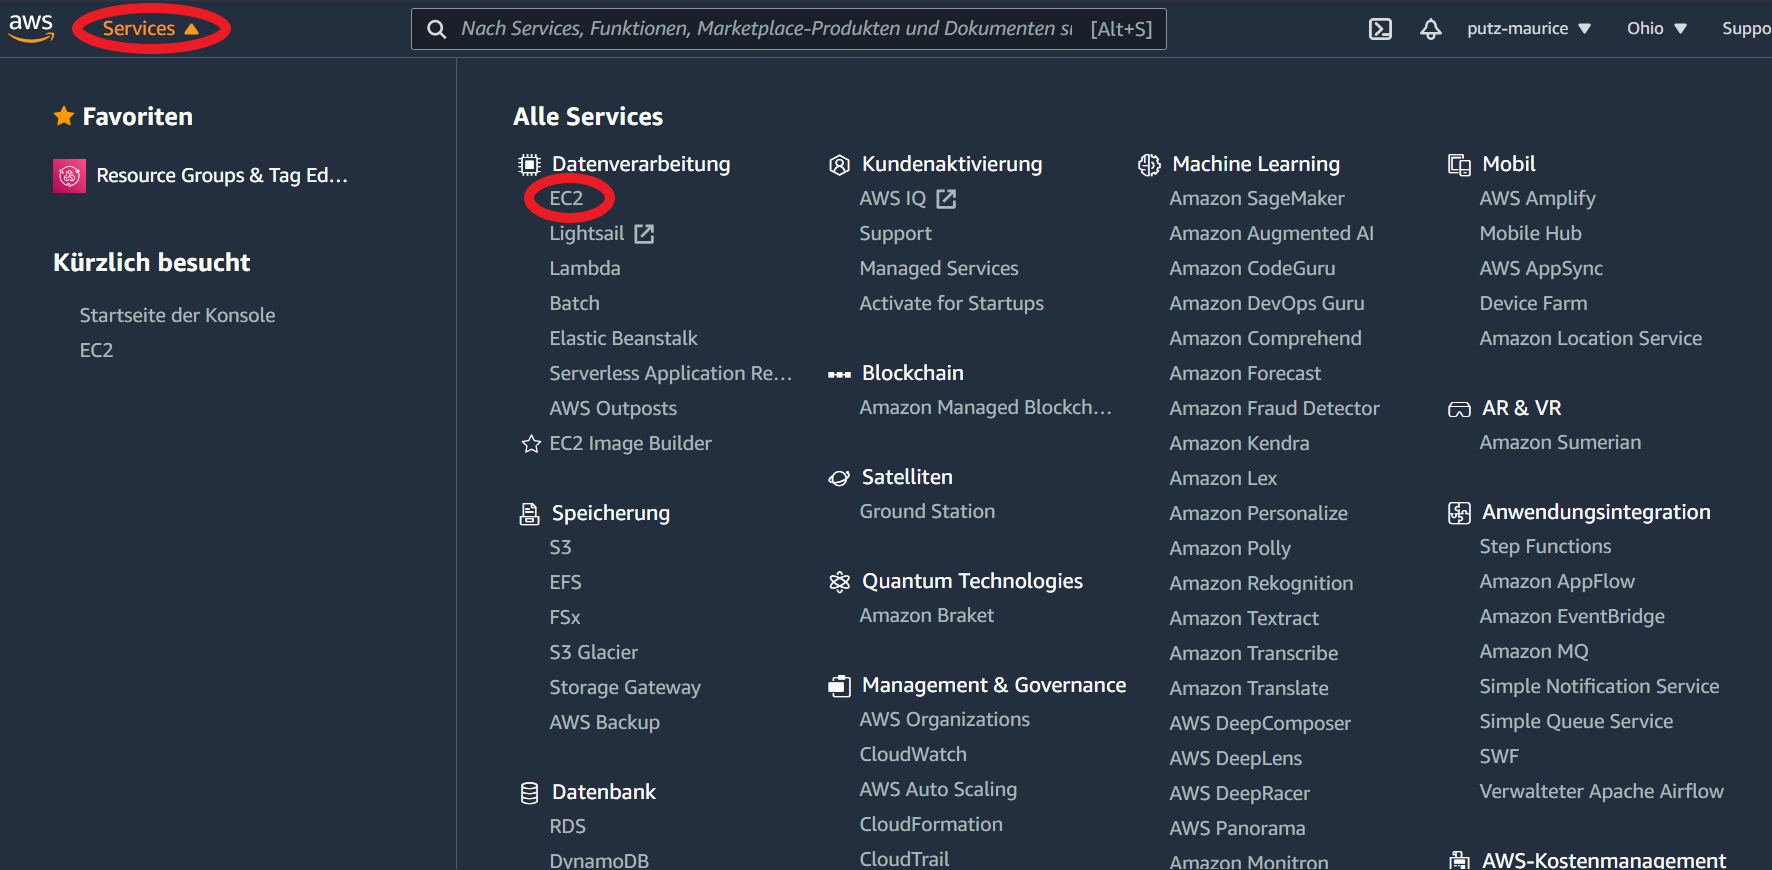
\includegraphics[width=\textwidth]{aws1.png}
    \caption{AWS Services Auflistung}
\end{figure}
\end{center}

Nachdem man die den EC2 Service ausgewählt hat, landet man auf dem EC2-Dashboard. Hier erhält man einen Überblick über alle laufenden Instanzen falls man schon bestehende hat, Load Balancer und weitere Services. Bevor man unten auf "´Instanz starten"' klickt, muss sichergestellt sein, dass man die richtige Region oben rechts ausgewählt hat. Dies hat vor allem Datenschutzrechtliche Gründe, grundsätzlich gilt, man wählt am besten das Land aus, aus welchem vor allem die Kunden daraus zugreifen. Man sollte, wenn man in einem Land, welches Mitglied in der EU ist, oder Daten von Benutzer aus der EU bei dem zu deployenden Programm anfallen, ein Land in der EU wählen. Zu sehen auf Abb. XX.

\begin{center}
\begin{figure}[h]
    \centering
    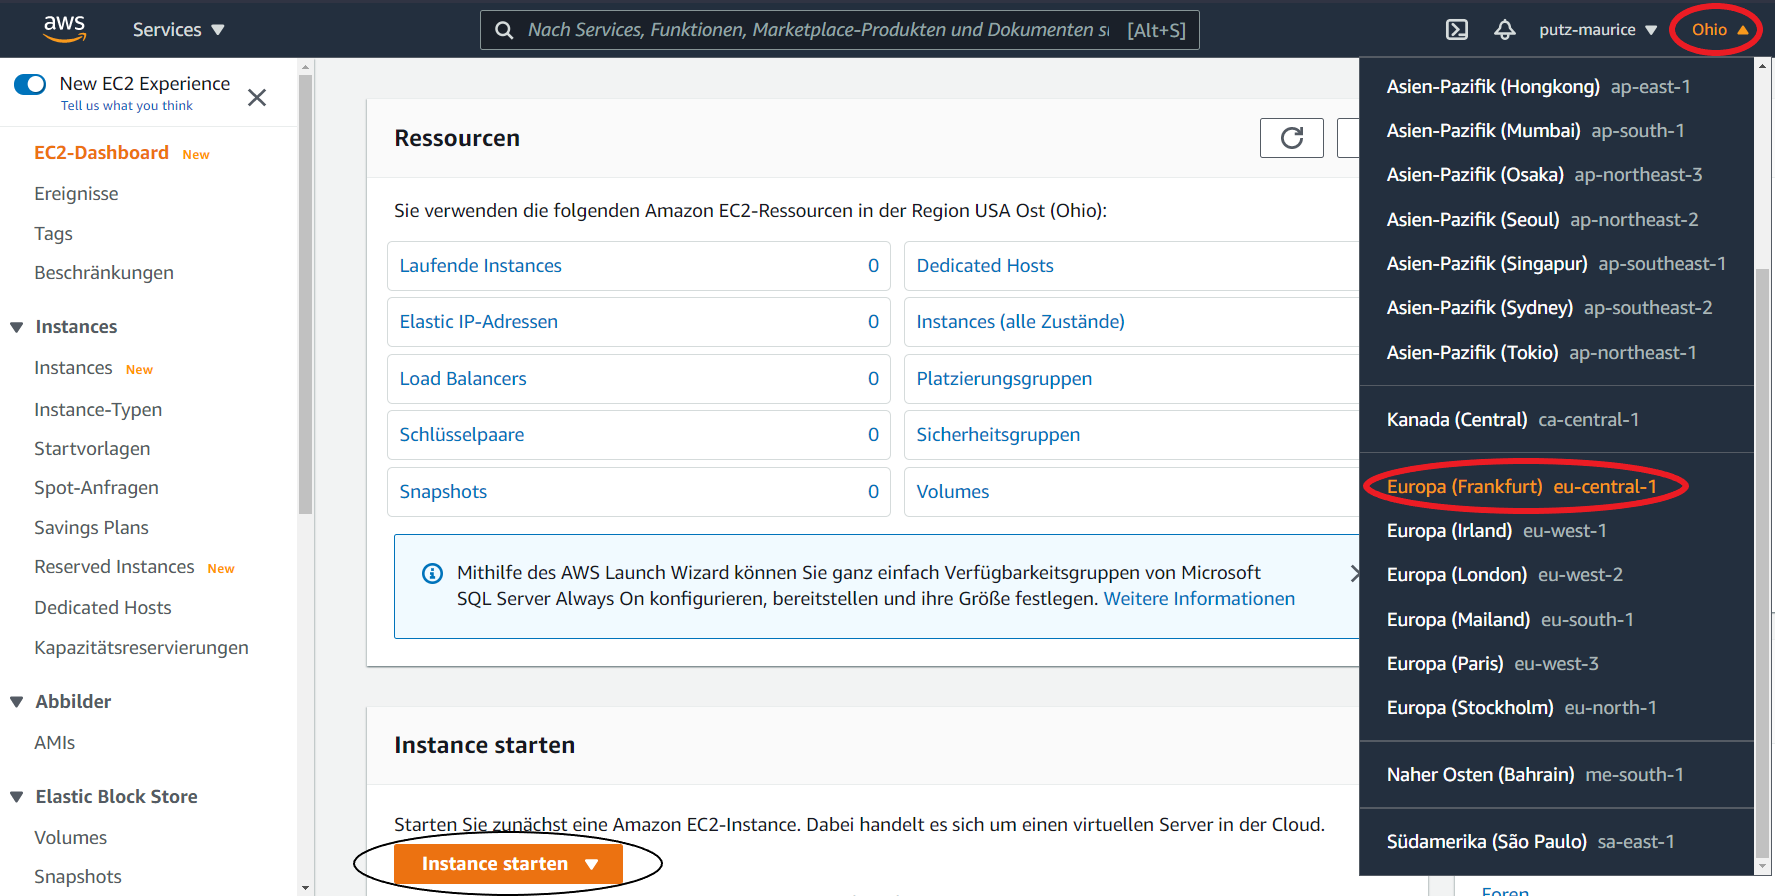
\includegraphics[width=\textwidth]{aws2.png}
    \caption{AWS Region ändern}
\end{figure}
\end{center}

Nach der Regionswahl, wird eine neue Instanz erstellt, nach entsprechendem Klick, startet der erste Schritt im Prozess. Zuerst wählt man ein Betriebssystem, worauf unser virtueller Server laufen wird. In unserem Fall war dies Ubuntu 20, da dies einen großen Marktanteil hat, alle Funktionen bietet welche wir benötigen und das OS gratis und uns bereits bekannt ist.

\begin{center}
\begin{figure}[h]
    \centering
    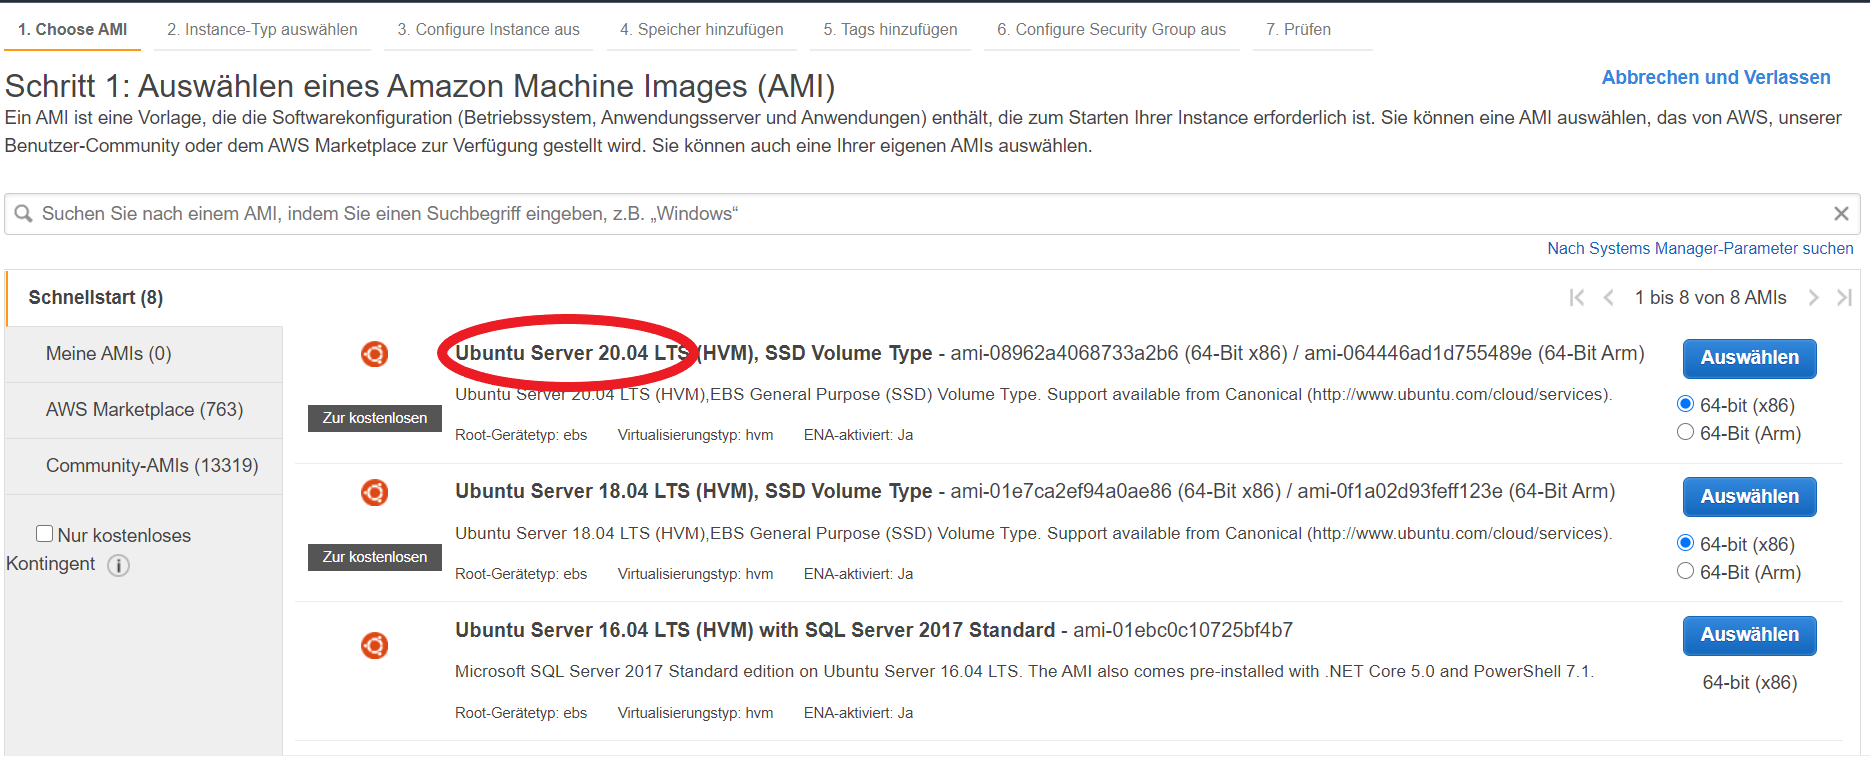
\includegraphics[width=\textwidth]{aws3.png}
    \caption{AWS OS auswählen}
\end{figure}
\end{center}

Der nächste Schritt beinhaltet das Selektieren des Instanz Typs. Wie viel virtuelle CPU's, wie viel RAM, wie viel Speicherplatz ohne zusätzliche Services wie zum Beispiel Amazon S3, der Serverinstanz später zu Verfügung steht. Wie gut die Netzwerkleistung ist und noch einige andere Details. Hier gibt es hunderte Instanzen, welche von zum Beispiel 1 Gigabyte RAM bis zu 3 Terrabyte RAM reichen. Für EMS reicht die gratis t2.micro Instanz. Die Spezifikationen dieser Instanz können aus Abb. XX entnommen werden. Diese Instanz kann jederzeit innerhalb von Minuten nach oben, beziehungsweise auch nach unten im Bezug auf Leistung, skaliert werden.

\begin{center}
\begin{figure}[h]
    \centering
    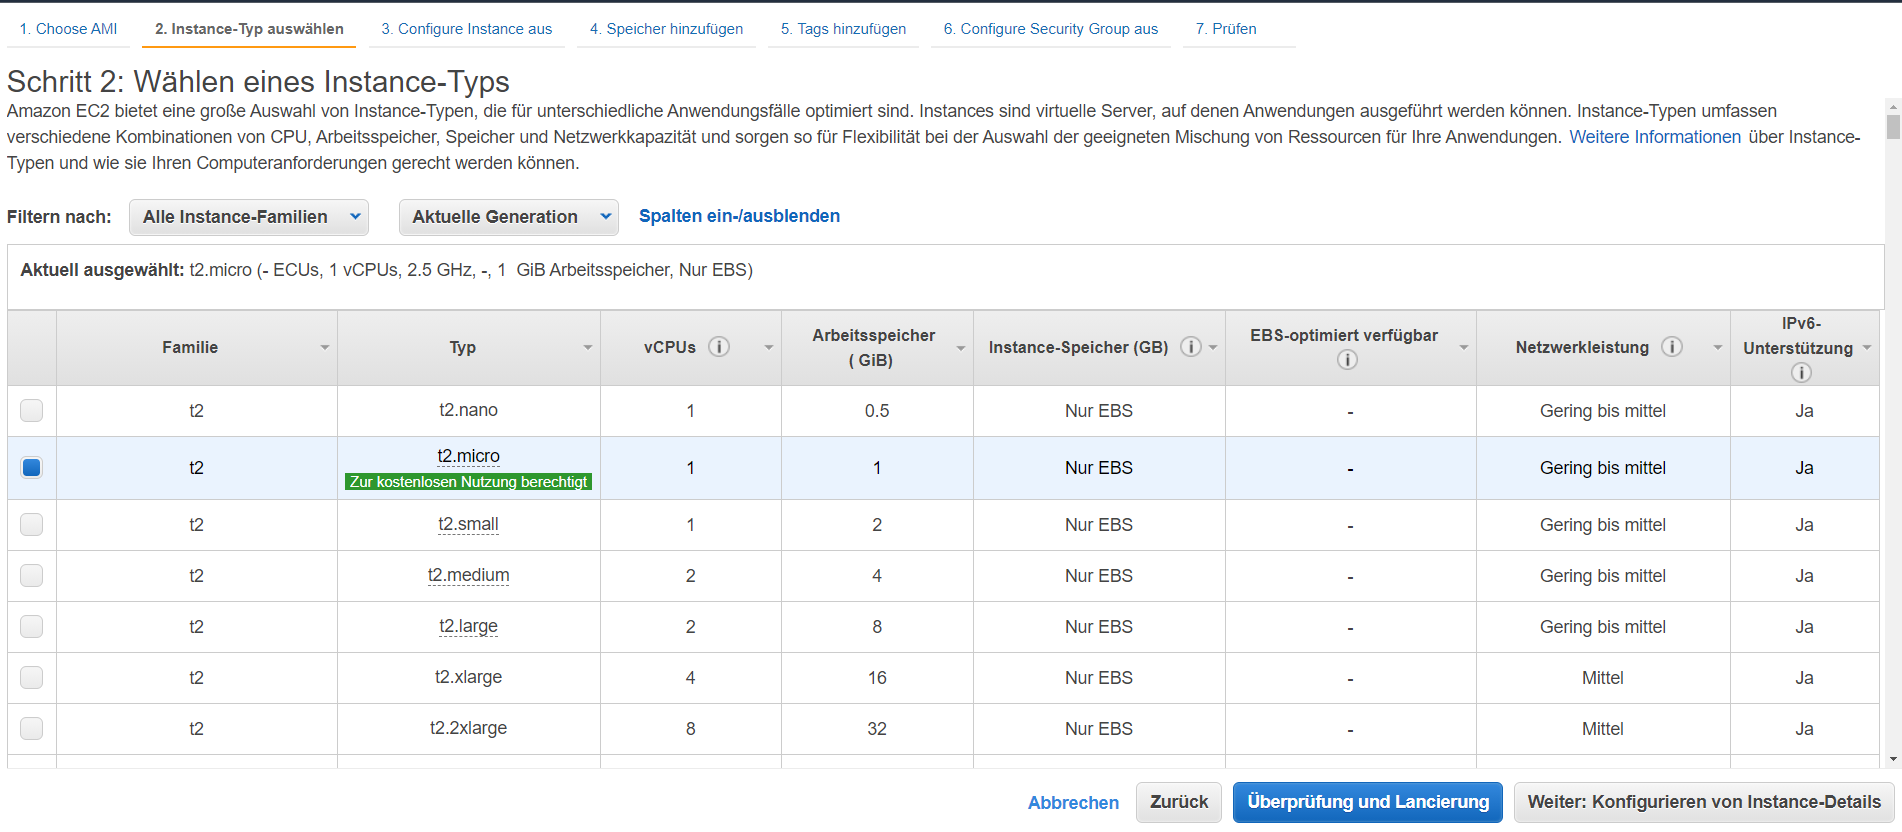
\includegraphics[width=\textwidth]{aws4.png}
    \caption{AWS Instanzspezifikationen}
\end{figure}
\end{center}

Im dritte Schritt werden die Anzahl der konfigurierten Anzahl eingeben und einige andere weitere Optionen, welche eine sehr feine Detailreiche und perfekt abgestimmte Instanz auf unterschiedlichste Use-Cases bietet. Für EMS sind auf dieser Seite keine weiteren Eingaben zum jetzigen Zeitpunkt nötig, da diese jederzeit im Nachhinein getroffen werden können und nicht alle auf der zuvor gewählten Instanz verfügbar sind. Auf dieser Seite kann man schon eine IAM-Rolle hinzufügen, dies sind die Benutzer in AWS, um auf eine EC2 Instanz über zum Beispiel SSH zuzugreifen oder Änderungen an der Instanz selbst vorzunehmen, muss man eine Rolle mit Berechtigungen erstellen, diese können dann später auch an andere Benutzer und AWS-Konten vergeben werden.

\begin{center}
\begin{figure}[h]
    \centering
    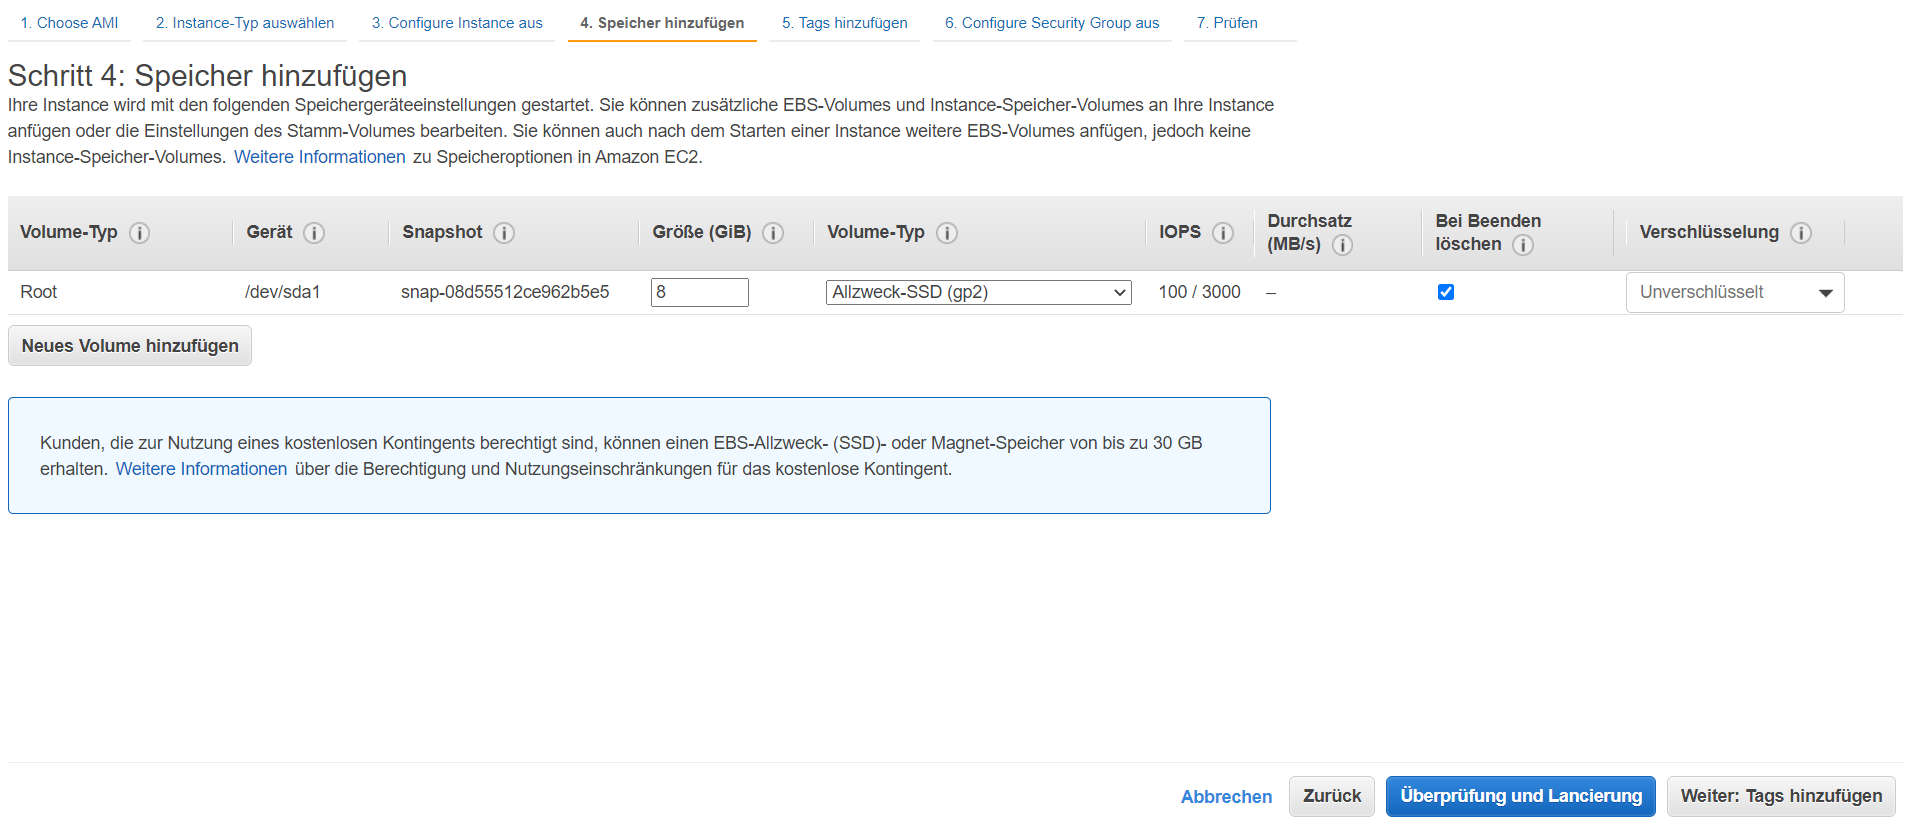
\includegraphics[width=\textwidth]{aws5.png}
    \caption{AWS Partitionierung}
\end{figure}
\end{center}

Im vierten Schritt wird die Größe des Speichers festgelegt. Optional kann dieser auf verschiedene Volumen verteilt werden und je nachdem, welchen Instanz Typ man in Schritt zwei ausgewählt hat, auch diese Verschlüsseln lassen. Sowie auch den Typ des Volumen, worauf alles gespeichert wird, läuft.

\begin{center}
\begin{figure}[h]
    \centering
    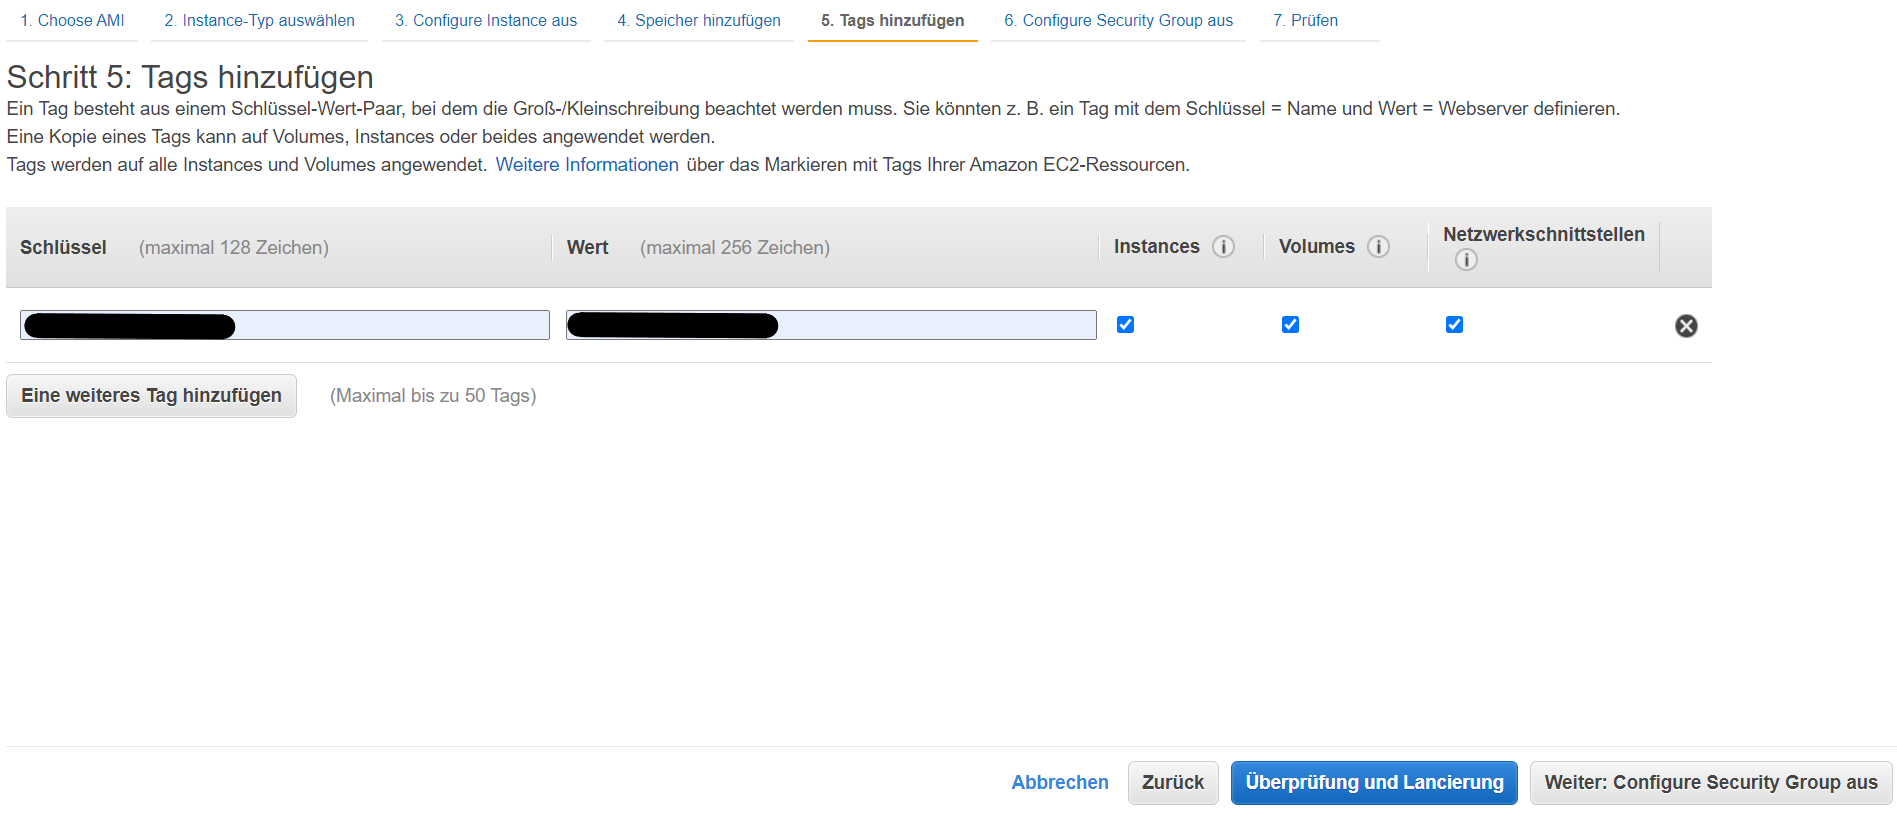
\includegraphics[width=\textwidth]{aws_tags.png}
    \caption{AWS Tags}
\end{figure}
\end{center}

Schritt Nummer fünf beinhaltet die Setzung von Tags für die Instanz. Diese werden in Key-Value Paaren angegeben. In Abb. XX ist aus Sicherheitsgründen der Schlüssel und der Wert zensiert, diese können komplett individuell und auf den Zweck der Instanz personalisiert sein.

\begin{center}
\begin{figure}[h]
    \centering
    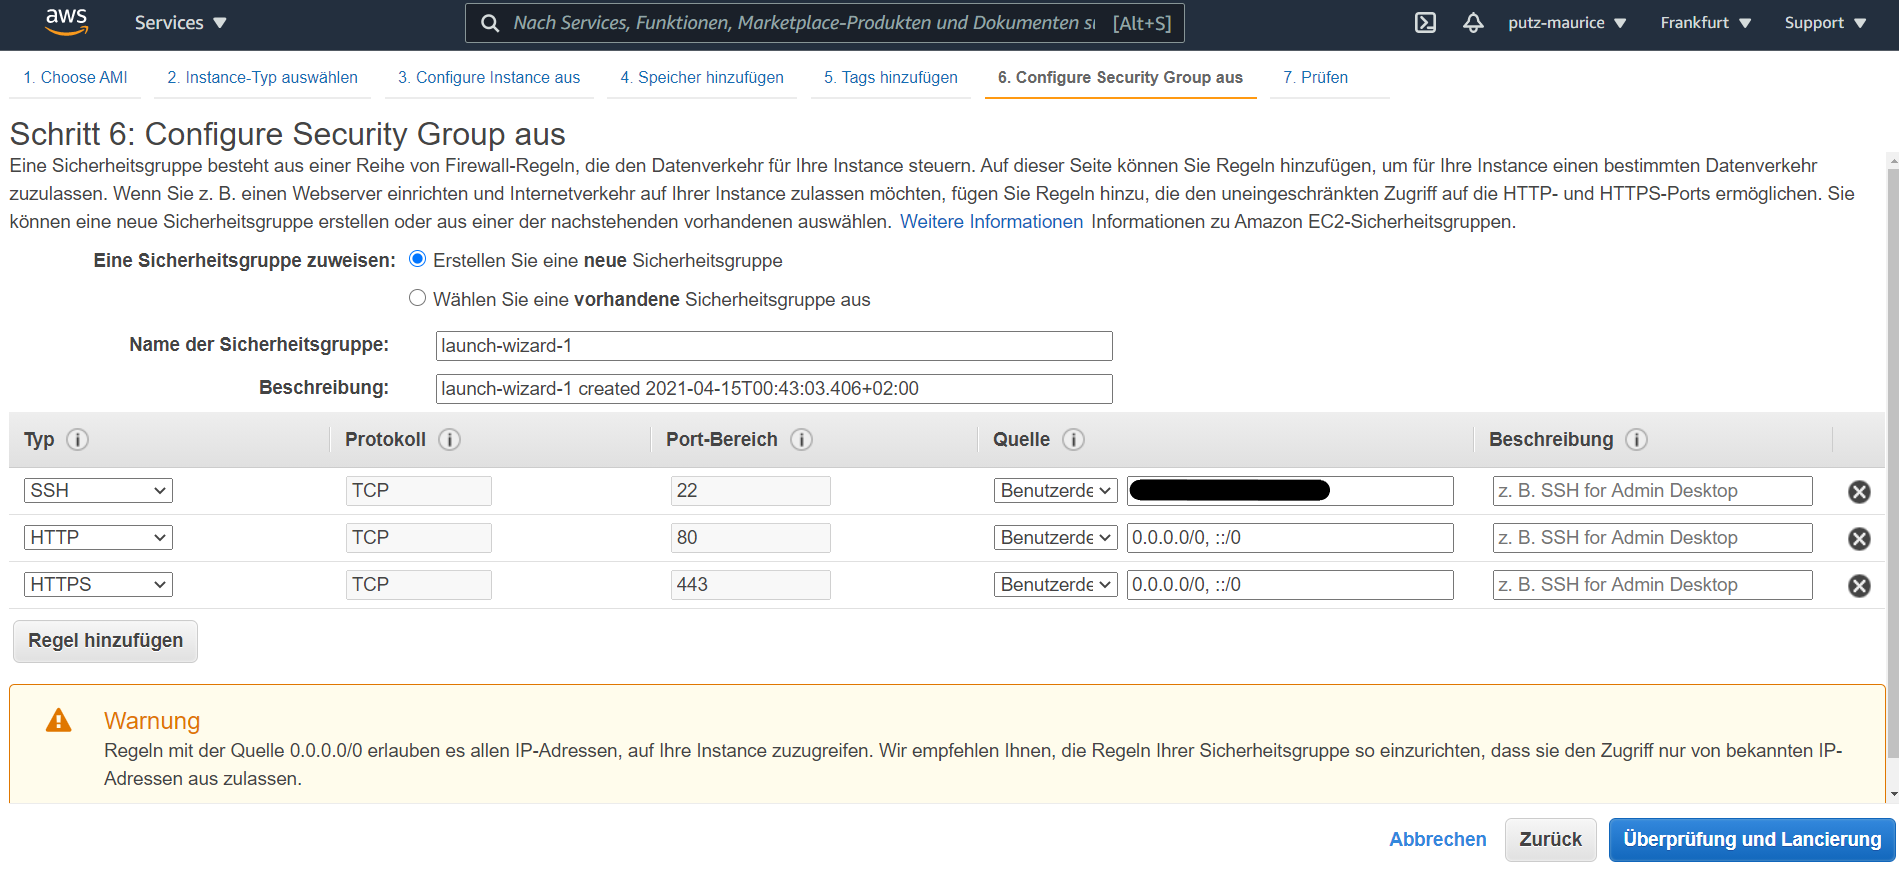
\includegraphics[width=\textwidth]{aws_security_group.png}
    \caption{AWS Sicherheit und Zugriff}
\end{figure}
\end{center}

Im sechsten und letzten aktiven Schritt zur Erstellung einer neue EC2 Instanz, fügt man Ports und Protokolle hinzu, welche für die Instanz geöffnet werden. Über diese Ports, kann dann direkt auf die Instanz zugegriffen werden, dies ist, damit das Backend von EMS mit der App oder der Webapp kommunizieren kann, essentiell. Die Protokolle wurde jeweils auf ihren Standardports laut IANA (Internet Assigned Numbers Authority). Wenn die zum Zugriff berechtigte Quelle auf den Standardwert \textbf{0.0.0.0/0} belassen wird, kann sich jede Quelle mit der Instanz verbinden.
Das hier ein Backend gehostet wird, werden Port 80 (HTTP) und Port 443 (HTTPS) für Anfragen aus allen Quellen offen sein. Zugriff mittels SSH auf Port 22 wird auf eine aus Sicherheitsgründen zensierte IP-Adresse beschränkt.

Nach der Auswahl der Zugriffspunkte und Ports, gelangt man auf eine Übersichtsseite. Hier kann man seine Angaben noch einmal überprüfen, sind alle Angaben korrekt, klickt man auf Start und in ein paar Minuten, die Zeit hängt von gewählter Option in Schritt zwei ab, ist die neue Instanz einsatzbereit und man kann sich zum Beispiel per SSH mit einer Shell (Putty) verbinden und zu arbeiten beginnen. 

\subsection{Backend deployment auf einer EC2 Instanz}
Nach der ersten Verbindung, müssen alle notwendigen Pakete und Anwendungen installiert werden, in unserem Fall Node.js und Express. Man kann direkt von Github ein Repository auf eine EC2 Instanz klonen. Sicherheitskritische Details wie IP-Adressen werden geschwärzt und zensiert.

\begin{center}
\begin{figure}[h]
    \centering
    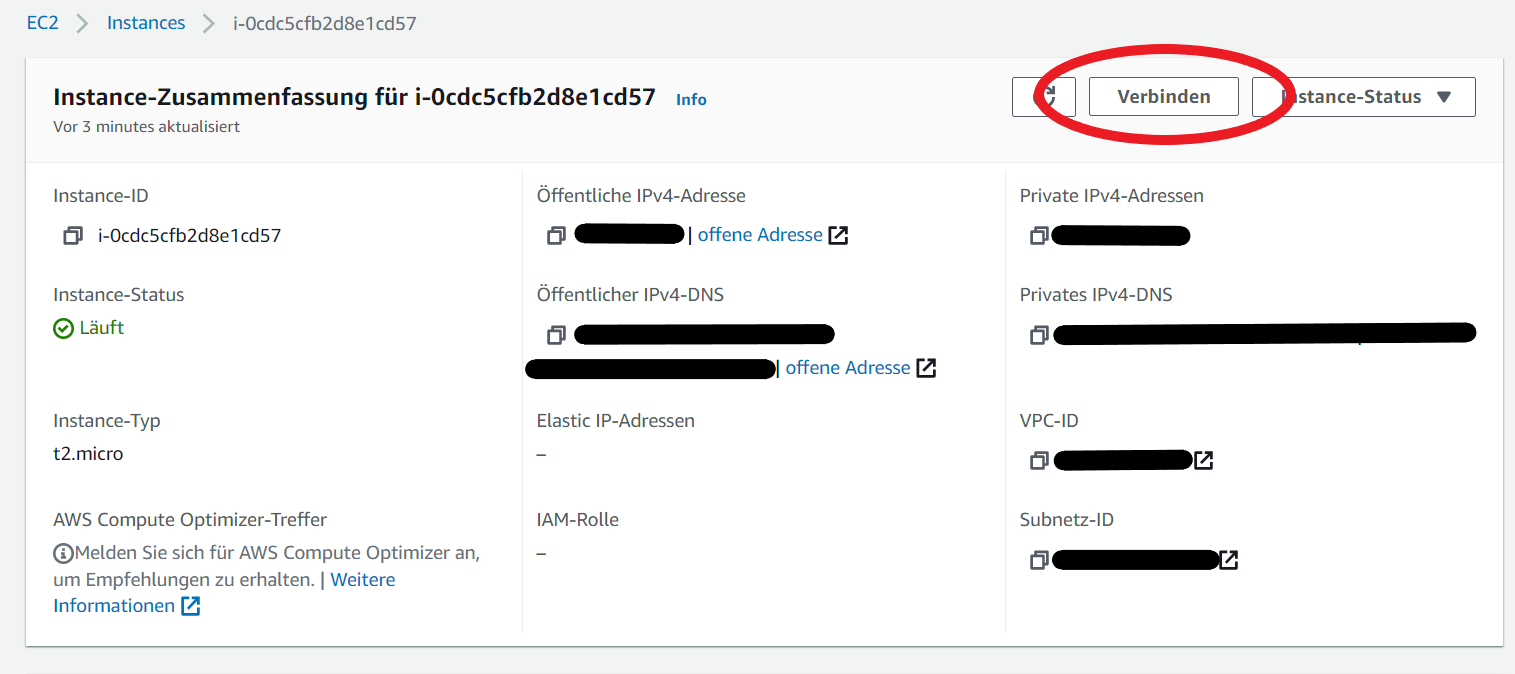
\includegraphics[width=\textwidth]{aws_verbinden.png}
    \caption{AWS Instanz Übersicht}
\end{figure}
\end{center}

In Abb. XInstanzÜX werden sämtliche Details der nun voll einsatzbereiten Instanz dargestellt, vorerst ist nur der Verbinden-Knopf rechts oben wichtig, hiermit kann man direkt eine SSH Verbindung mit seiner Instanz herstellen, ohne seinen .pem Schlüssel, welchen man bei erstellen der Instanz am Ende herunterladen musste, zu nutzen. Eine einfache, sichere und schnelle Methode um über eine Shell auf der Instanz zu arbeiten.

\begin{center}
\begin{figure}[h]
    \centering
    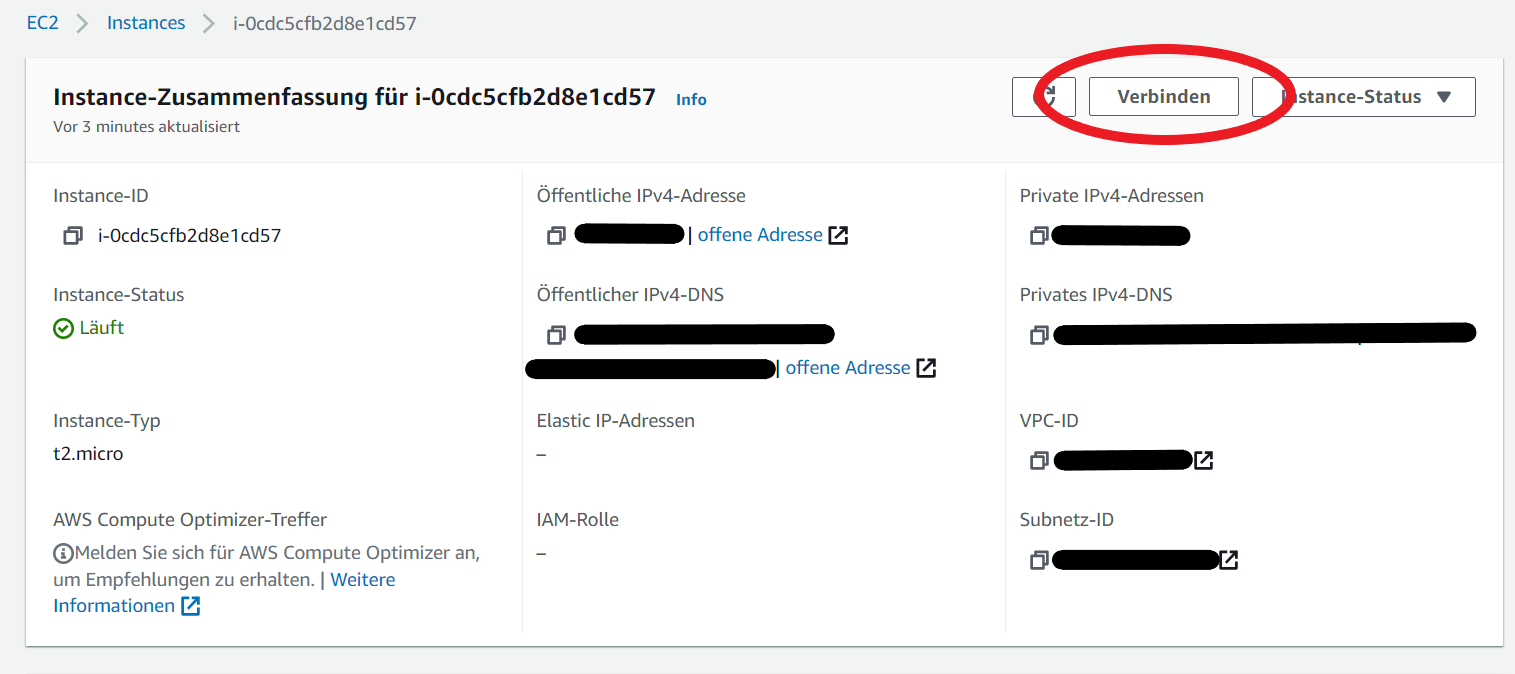
\includegraphics[width=\textwidth]{aws_verbinden.png}
    \caption{AWS SSH Verbindung}
\end{figure}
\end{center}

Nun mit der Instanz verbunden, muss, um einen Node.Js Server zu hosten, zuerst Node.Js und installiert werden, da in dem Beispiel hier ein komplettes Backend mit Express gehostet wird, muss dies auch installiert werden. Dies kann unter Ubuntu 20 mit den folgenden Befehlen in angegebener Reihenfolge gemacht werden:

\begin{lstlisting}[language=bash]
# Using Ubuntu and Node.js Version 15+
curl -fsSL https://deb.nodesource.com/setup_15.x | sudo -E bash -
sudo apt-get install -y nodejs

#For newest Express version
sudo npm install -g express-generator

#For nodemon
sudo npm i -g nodemon
\end{lstlisting}

Nach erfolgreicher Installation sollte mit mit in Abb. XX zu sehendem Kommando, die aktuelle Node.Js Version Installation überprüfen können. (Falls die Installation nicht erfolgte, überprüfen ob man den Befehl sudo benutzt hat.)

\begin{center}
\begin{figure}[h]
    \centering
    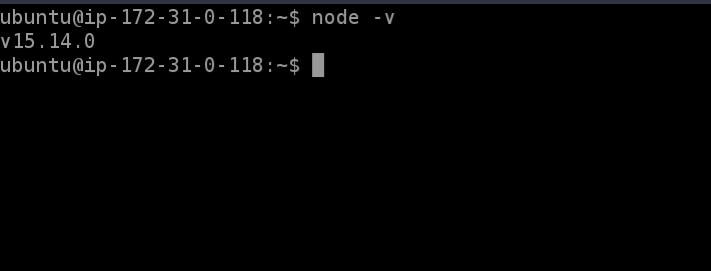
\includegraphics[width=\textwidth]{aws_nodejs_v.png}
    \caption{AWS Node.js Version}
\end{figure}
\end{center}

Unter Ubuntu musst Git nicht installieren werden, da es mitausgeliefert wird. Falls dies aber doch der Fall sein sollte, kannst man es mit folgendem Befehl installieren;

\begin{lstlisting}[language=bash]
sudo apt-get install git
\end{lstlisting}

Danach klont man das Git-Repository mit dem Backend oder der Node.js Anwendung auf die AWS Instanz.


\begin{lstlisting}[language=bash]
git clone https://github.com/[PATH_TO:REPOSITORY]
\end{lstlisting}

Nach sämtlichen Installationen und wechseln in das Verzeichnis des Repositories, wird das Backend gestartet, dies geschieht mit folgenden Befehlen:

\begin{lstlisting}[language=bash]
npm install

nodemon start
\end{lstlisting}

\begin{center}
\begin{figure}[h]
    \centering
    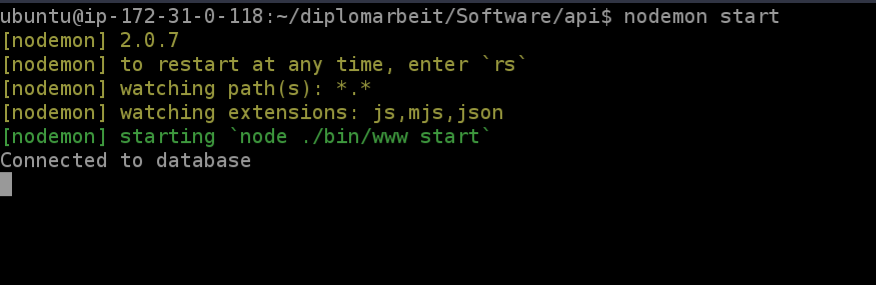
\includegraphics[width=\textwidth]{aws_nodejs_s.png}
    \caption{AWS Backend running}
\end{figure}
\end{center}

Abb. zeigt einen Node.js und Express Server auf einer AWS EC2 Instanz laufend. Der Server läuft jetzt auf Port 3000. Wenn man nun aber die öffentliche DNS Adresse der Instanz in die Suchleiste eines Webbrowser einfügt und den Port des Server noch dazu angibt, passiert noch nichts, obwohl die Instanz und Node.js online sind. Damit der Server auch von außerhalb der Instanz erreicht werden kann, muss entsprechender Port geöffnet werden.

\begin{center}
\begin{figure}[h]
    \centering
    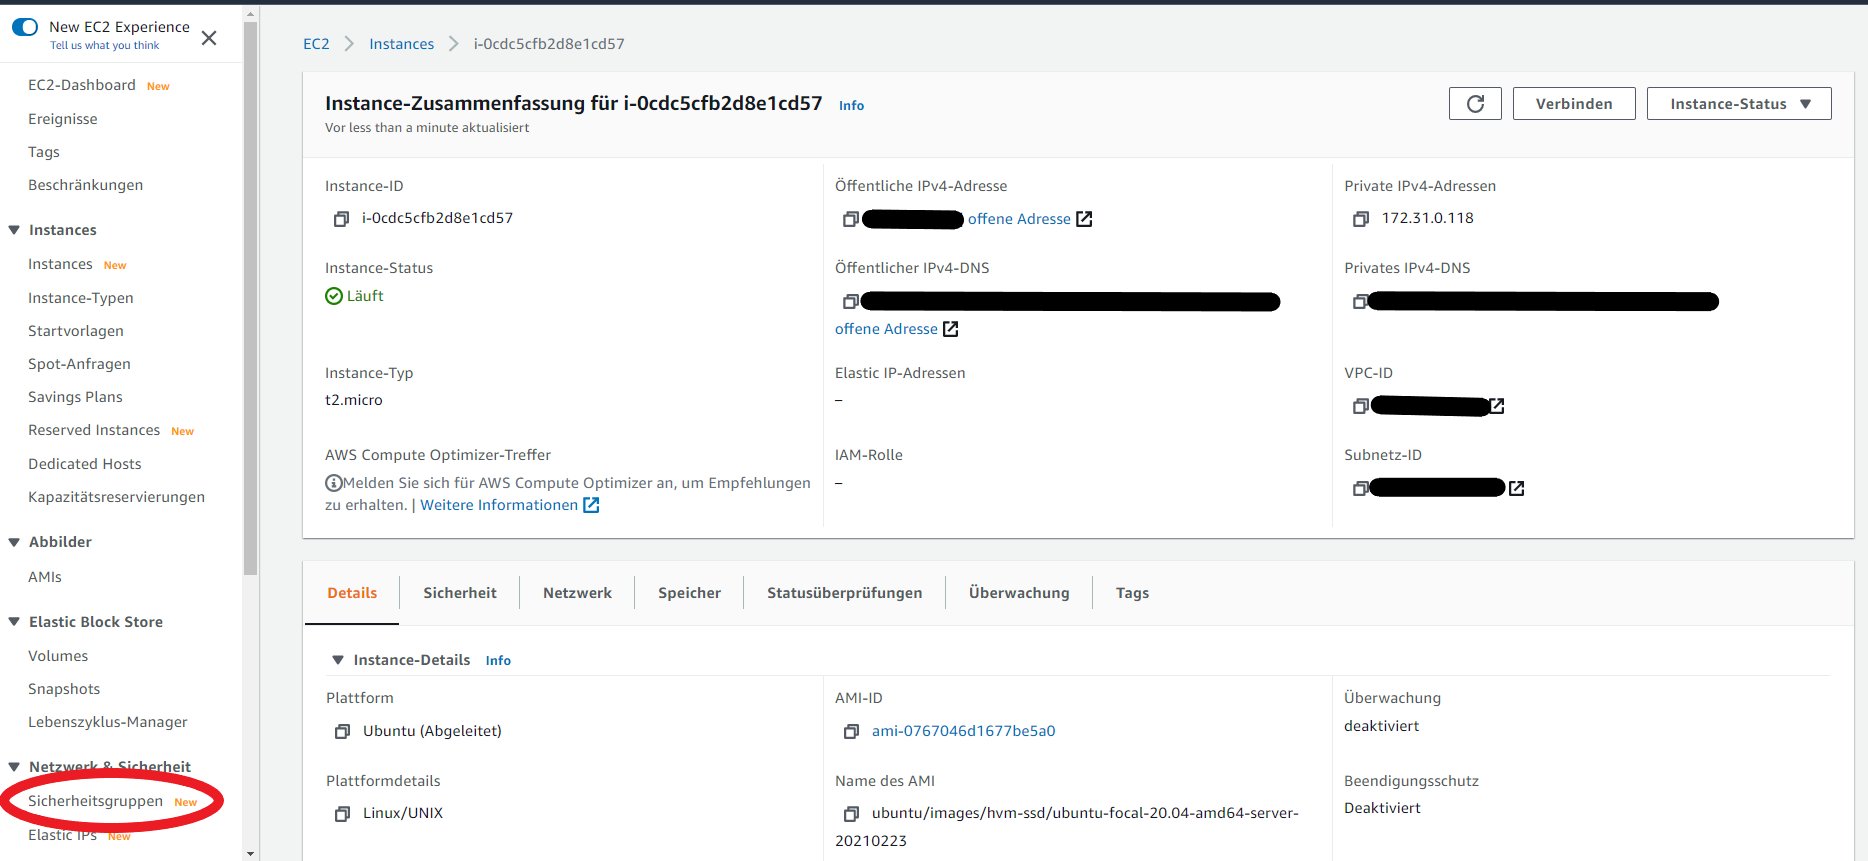
\includegraphics[width=\textwidth]{aws_nodejs_sicherheitsgruppe.png}
    \caption{AWS Dashboard Sicherheitsgruppe auswählen}
\end{figure}
\end{center}

Dies geschieht in dem man auf de, EC2 Dashboard auf "`Sicherheitsgruppen"' geklickt hat, wie in Abb. XX zu sehen ist. 

\begin{center}
\begin{figure}[h]
    \centering
    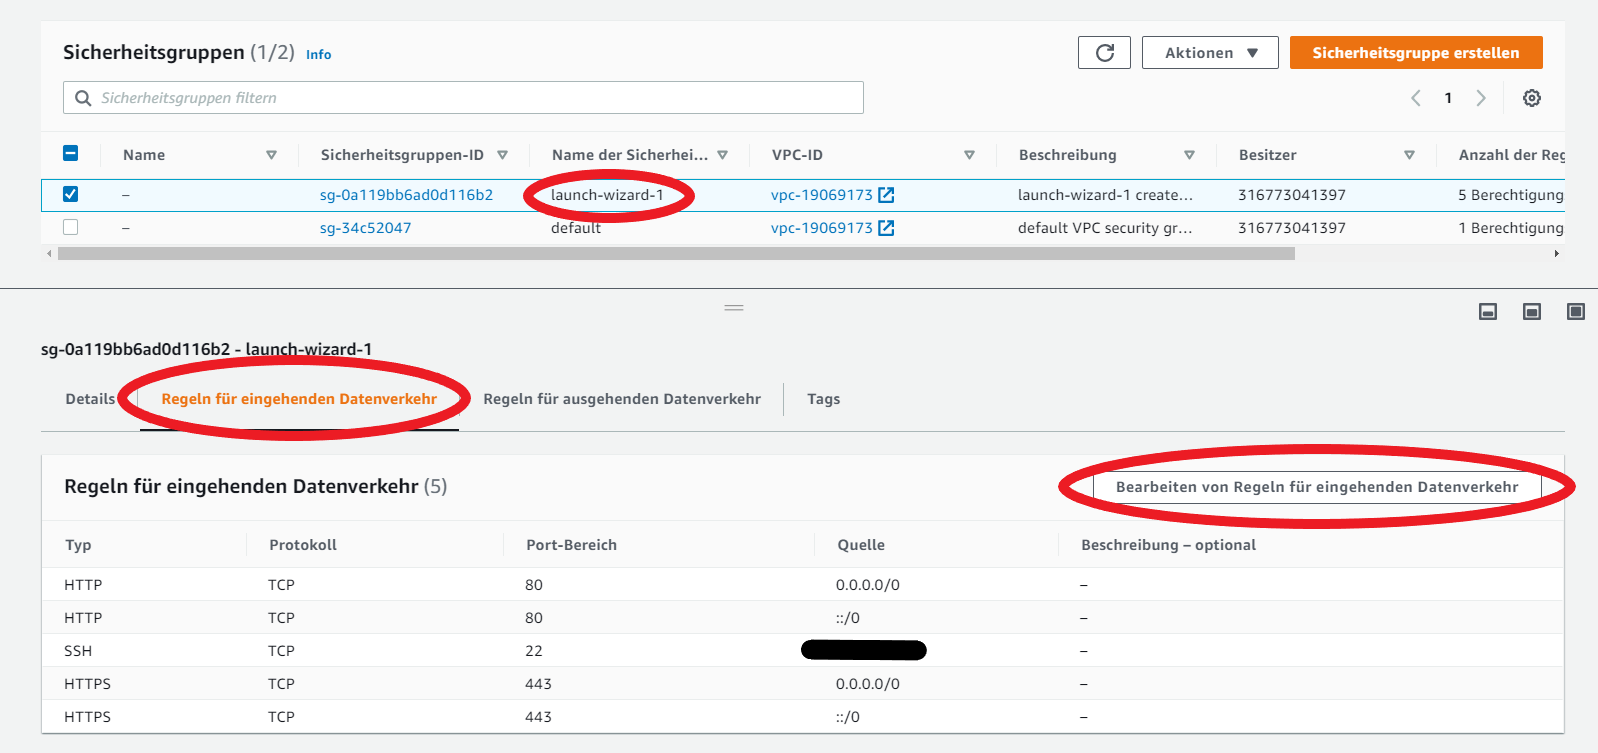
\includegraphics[width=\textwidth]{aws_launch_wizard.png}
    \caption{AWS Dashboard Sicherheitsgruppe auswählen}
\end{figure}
\end{center}

Bei der Erstellung der Instanz, hat man gleichzeitig auch eine Sicherheitsgruppe erstellt, unter Schritt sechs. Diese wird nun ausgewählt und im unteren Fenster der Reiter "´Regeln für eingehenden Datenverkehr"' ausgewählt und dort auf Bearbeiten geklickt.


\begin{center}
\begin{figure}[h]
    \centering
    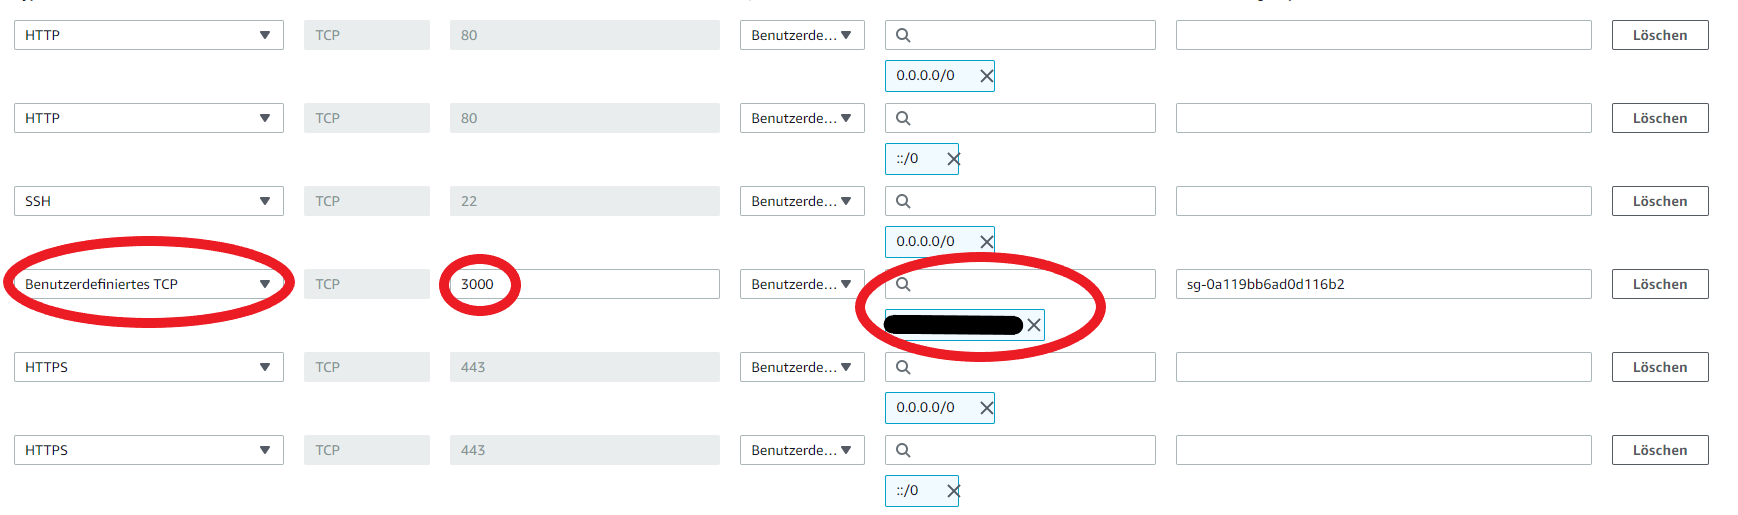
\includegraphics[width=\textwidth]{aws_ports_ende.png}
    \caption{AWS Dashboard Sicherheitsgruppe auswählen}
\end{figure}
\end{center}

Eine Neue Regeln hinzufügen und den Port des Node.js/Express Servers eingeben, plus als Quelle die Sicherheitsgruppen ID der gewählten Sicherheitsgruppe eintragen, dies bewirkt dass alles Instanzen mit dieser Sicherheitsgruppe Port 3000 frei haben.

Indem man nun bis zu maximal einer Minute wartet, damit alle Änderungen übernommen worden sind, kann der Server über Port 3000 aufgerufen werden und Funktionen ausgeführt werden zum Beispiel:

\begin{lstlisting}[language=bash]
http://[Oeffentlicher-IPv4-DNS-DER-INSTANZ].compute.amazonaws.com:[PORTNUMMER]/[FUNKTIONS_NAME]
\end{lstlisting}

Die Ausgabe erscheint dann im unteren Bereich, falls die Funktion einen Rückgabewert besitzt, wie in Abb. zu sehen.

\begin{center}
\begin{figure}[h]
    \centering
    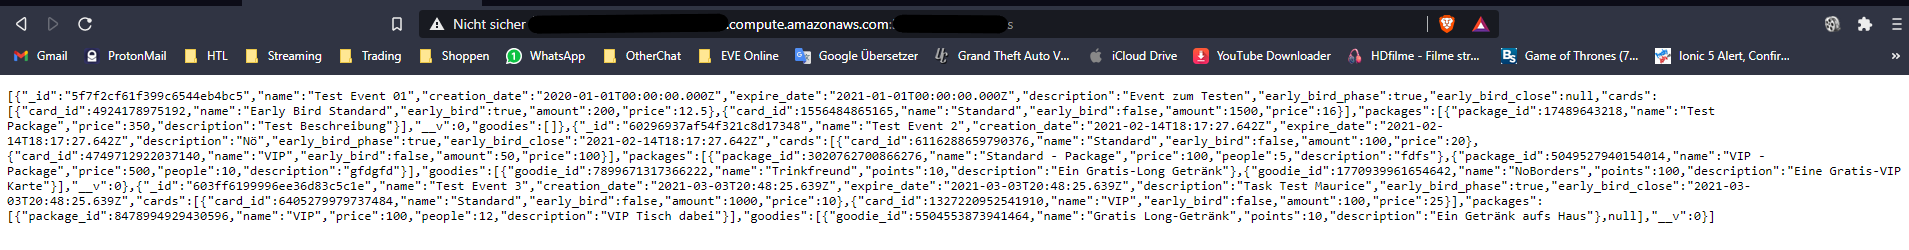
\includegraphics[width=\textwidth]{aws_functionsaufruf.png}
    \caption{AWS Instanz Port geöffnet}
\end{figure}
\end{center}

Einen letzten Schritt gibt es noch. Der Server läuft in einem SSH Fenster im Vordergrund und kann mit Strg+C abgebrochen werden. Um den Prozess nun im Hintergrund laufen zu lassen, gibt man folgenden Befehl ein:

\begin{lstlisting}[language=bash]
#Installieren von pm2
sudo npm install pm2 -g

#Zum starten im Hintergrund, in bin Ordner wechseln und
sudo pm2 start www

#Zum anzeigen aller Prozesse in pm2
sudo pm2 list
\end{lstlisting}

Die Ausgabe wie in Abb. XX zu sehen ist, zeigt den Prozess in pm2 unter der OS - Prozess ID 4165 und pm2 ID 1 laufen. Er ist online und einige weitere Details zur Analyse und Fehlerbehandlung werden angezeigt. Sollte man am Server im Code ändern, muss man den Hintergrundprozess neu starten. Dies geht mit:

\begin{lstlisting}[language=bash]
#Neustart von pm2 Prozess mit ID 1
sudo pm2 restart 1

#Stoppe Prozess
sudo pm2 stop 1
\end{lstlisting}

\begin{center}
\begin{figure}[h]
    \centering
    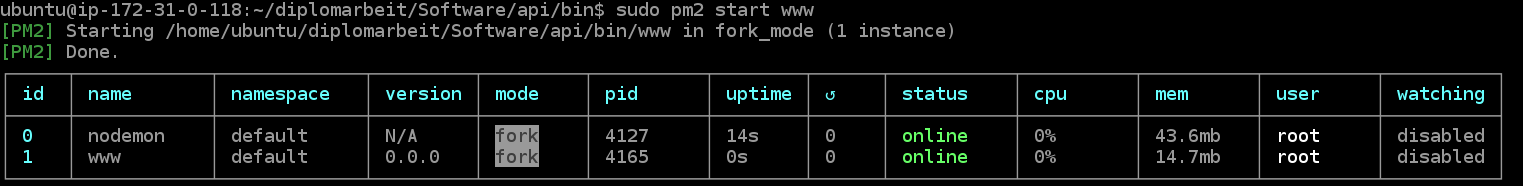
\includegraphics[width=\textwidth]{aws_om2.png}
    \caption{AWS Node.js Server im Hintergrund}
\end{figure}
\end{center}


\newpage
 